\section{Grundlagen} % (fold)
\label{sec:grundlagen}

	\subsection{Interferenz und Kohärenz} % (fold)
	\label{sub:interferenz_und_koh_renz}
		
		Bringt man zwei Teilbündel der selben Lichtquelle zur Überlagerung (wie hinter einem Youngschen Doppelspalt) kommt es zur Addition der Feldstärken. 
		Weisen beide Teilbündel die gleiche Polarisation auf, was im Normalfall ohne Bauelemente die die Polarisation beeinflussen zutrifft, so kommt es am Ort der Überlagerung zu Interferenzerscheinungen, wenn die Teilbündel eine Phasendifferenz $\varphi$ besitzen.
		Da nur gleich polarisiertes Licht interferieren kann, wird die elektrische Feldstärke $E$ im folgenden immer als skalare Größe behandelt.
		\[ E_1(t) = \hat{E}_1 \cos(\omega t),\qquad E_2(t) = \hat{E}_2 \cos(\omega t + \varphi) \]%
		Für die Intensität der interferierenden Strahlen folgt dann:
		\begin{alignat*}{3}
			\implies \quad I &=&&\ \overline{\boxb{E_1(t) + E_2(t)}^2} \\
				&=&&\  \hat{E}^2_1\ \overline{\cos^2(\omega t)} + \hat{E}^2_2\ \overline{\cos^2(\omega t)} \\
				& &&\ + 2\hat{E}_1 \hat{E}_2\ \overline{\cos(\omega t)\cos(\omega t + \varphi)}
		\end{alignat*}
		Für den zeitlich gemittelten Anteil gilt nun:
		\begin{alignat*}{3}
			\overline{\cos(\omega t)\cos(\omega t + \varphi)} &=&&\ \overline{\cos(\omega t)\boxb{\cos (\omega t) \cos \varphi - \sin (\omega t) \sin \varphi } }\\
				&=&&\ \overline{\cos^2 (\omega t) \cos \varphi} - \overline{\cos (\omega t) \sin (\omega t) \sin \varphi} \\
				&=&&\ \tfrac{1}{2}\cos \varphi
		\end{alignat*}
		 \[ \implies \quad I = I_1 + I_2 + 2 \sqrt{I_1 I_2} \cos \varphi \]
		 Für gleiche Intensitäten $I_1 = I_2 = I_0$ kann die Formel vereinfacht werden:
		 \[ I = 2 I_0 + 2 I_0 \cos\varphi = 2 I_0 \curvb{1 + \cos\varphi} \]

		 Voraussetzung für die Interferenz von Lichtstrahlen ist ihre Kohärenz.
		 Zwei Teilwellen werden kohärent genannt, wenn sie über eine konstante Phasendifferenz in Beziehung stehen.
		 Man unterscheidet räumliche und zeitliche Kohärenz.
		 Die Kohärenzzeit $t_\m{koh} $ ist die Spanne, in der sich die Phasendifferenz nicht ändert, bzw. genauer, in der sie sich um weniger als $2 \pi $ ändert.

		 Jeden Wellenzug kann man als eine Überlagerung monochromatischer Schwingungen, also als seine Fouriertransformation darstellen:

		 \[ E(\vec{r}, t) = \Integral{f_0-\Delta f/2}{f_0+\Delta f/2}{ \tilde{E}(\vec{r}, \omega) e^{-i \omega t} }{\omega} \]

		 Nach den Regeln der Fouriertransformation ist ein Wellenzug nun zeitlich umso kürzer, je breiter sein Spektrum, d.h. je größer $\Delta f$ ist.
		 Da zwei Wellenzüge generell inkohärent sind, ist also die Kohärenzlänge $t_\m{koh}$ maximal so lang wie ein Wellenzug.
		 Es gilt der einfache Zusammenhang:

		 \[ t_\m{koh} = \frac{1}{\Delta f} \]

		 Streng monochromatische Strahlung hat demnach als Fouriertransfomierte einen Delta-Peak und eine unendliche Kohärenzzeit und -länge.
		 Die Kohärenzlänge $l_\m{koh}$ ergibt sich mit der Phasengeschwindigkeit $c$ zu:

		 \[l_\m{koh} = c\ t_\m{koh} \]

	% subsection interferenz_und_koh_renz (end)


	\subsection{Prinzip des Michelson-Interferometers} % (fold)
	\label{sub:prinzip_des_michelson_interferometers}

		\urldef{\mifscheme}\url|https://upload.wikimedia.org/wikipedia/commons/thumb/b/b0/Michelson_interferometer_white_light.svg/2000px-Michelson_interferometer_white_light.svg.png|

		\begin{figure}[htb]
			\centering
			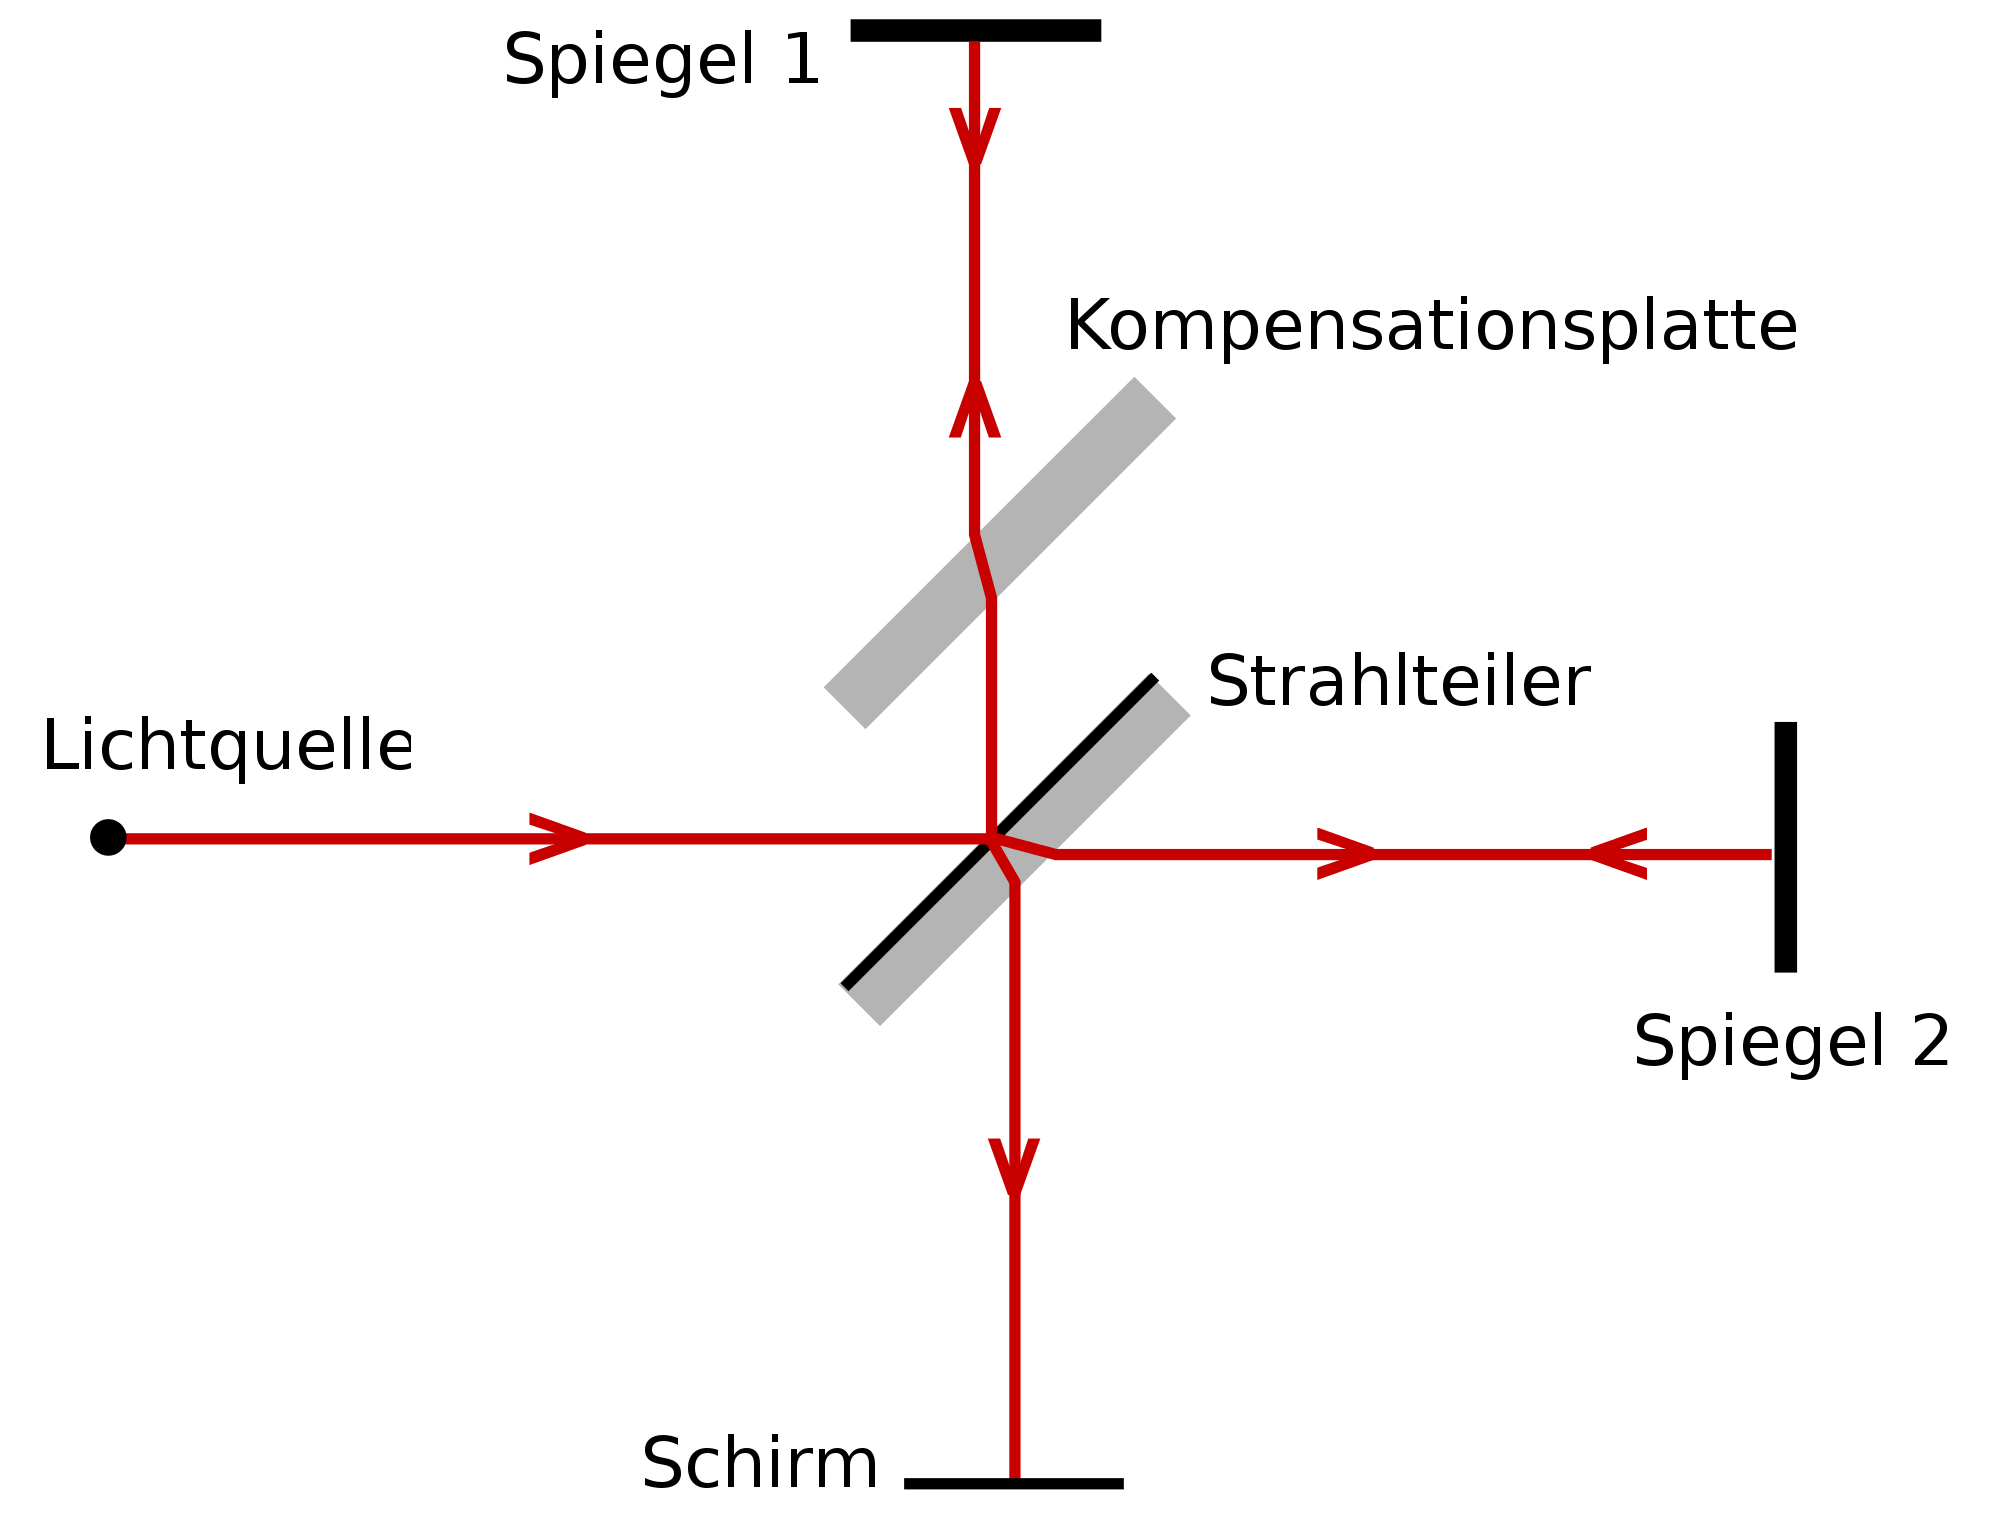
\includegraphics[scale=0.16]{images/mif-schema.png}
			\caption{Schema zum Aufbau des verwendeten Michelson-Interferometers \\ Quelle: \\ \mifscheme}
			\label{fig:grundlagen-mif-schema}
		\end{figure}

		Wie in Abbildung \ref{fig:grundlagen-mif-schema} zu sehen, durchläuft das Licht im Michelson-Interferometer (MIF) ausgehend von der Quelle zunächst den Kollimator um dann auf einen 50/50-Strahlteiler zu treffen, der zwei Bündel möglichst gleicher Intensität zu den Spiegeln Spiegel 1 und Spiegel 2 führt.
		Je genauer die beiden Intensitäten übereinstimmen, desto größer ist der Kontrast zwischen Interferenzminimum und -maximum. 
		Spiegel 2 ist verstellbar und somit kann die optische Wegdifferenz der beiden Teilstrahlen beliebig eingestellt werden.
		Nach erneuter Ablenkung durch den Strahlteiler gelangt der eine Teil der Lichtbündel zurück zur Quelle, der andere erreicht den Ausgang und wird über das Objektiv auf eine Fläche abgebildet.
		Je nach Art des Strahlteilers kann eine Kompensationsplatte in einem der beiden Strahlengänge erforderlich sein, um zu verhindern, dass nur einer der Teilstrahlen z.B. eine Strecke in Glas zurücklegt und so von vorneherein eine ungewollte Wegdifferenz aufweist.
		Beträgt die Spiegelverschiebung $\Delta x$ weniger als die halbe Kohärenzlänge, so lassen sich auf dem Schirm je nach Stellung der Spiegel unterschiedliche Interferenzerscheinungen einstellen und beobachten.
	
	% subsection prinzip_des_michelson_interferometers (end)

	\subsection{Interferenzen gleicher Neigung} % (fold)
	\label{sub:interferenzen_gleicher_neigung_haidinger_ringe}

		Bei idealen Bauteilen und idealer Justierung, d.h. plane Spiegel, keine Verzeichnung durch Linsen und Kollimator, exakt rechtwinklige Ausrichtung der Spiegel, homogenen Strahlenbündel usw. sind auf dem Schirm konzentrische Kreise zu erkennen, genannt Haidinger Ringe.
		Analog lasssen sich zwei Lichtquellen L1 und L2 im Abstand $2 \Delta x$ auf einer Achse vor dem Schirm betrachten.
		Maxima lassen sich nun an allen Stellen finden, wo die Phasendifferenz $\varphi = 2 \pi$ beträgt, also der Wegunterschied gleich $\lambda$ ist.
		Bei gleichmäßiger Erhöhung von $\Delta x$ ziehen sich die Ringe zusammen, veringert man den Wegunterschied, quellen sie auseinander.

	% subsection interferenzen_gleicher_neigung_haidinger_ringe (end)


	\subsection{Interferenzen gleicher Dicke} % (fold)
	\label{sub:interferenzen_gleicher_dicke_fizeau_streifen}
	
		Wenn beide Spiegel in etwa die gleiche Weglänge aufweisen, so kann man durch Verkippen des einen Interferenzen gleicher Dicke, sogenannte Fizeau-Streifen erzeugen.
		Die gleichen Muster treten bei zwei ebenen Wellen auf, die im Winkel $\alpha$ zusammenlaufen.
		Aus einfachen geometrischen Überlegungen folgt für den Abstand $a$ zwischen zwei Maxima auf dem Schirm:

		\[ a = \frac{\lambda}{2 \sin\frac{\alpha}{2}} \]

		Die Gleichung berücksichtigt nur ebene Wellen und keine Skalierung durch abbildende Optik.
		Die Skalierung kann nachträglich z.B. durch vermessen der Bildgröße dirket nach dem Würfel oder durch Abmessen des Linsendurchmessers erfolgen.

	% subsection interferenzen_gleicher_dicke_fizeau_streifen (end)

	\subsection{Fourierspektroskopie} % (fold)
	\label{sub:fourierspektroskopie}
		
		Wie unter \ref{sub:interferenz_und_koh_renz} beschrieben gilt für die Intensität im Falle gleicher Strahlteilung:
		\[ I = 2 I_0 + 2  I_0 \cos\varphi \]
		Drücken wir die Phasendifferenz $\varphi$ durch die zeitliche Verschiebung $\tau$ aus, erhalten wir
		\[ \varphi = \omega \tau \]
		Die Intensität ist normalerweise über einen gewissen Frequenzbereich verteilt und lässt sich somit durch
		\[ I = \integral{0}{\infty}{i(\omega)}{\omega} \]
		ausdrücken.
		Dabei stellt $i(\omega)$ die spektrale Leistungsdichte dar.
		Ziel einer jeden Spektroskopie ist es genau diese Funktion möglichst breit und hoch aufgelößt zu bestimmen.
		Aus allen drei Formeln folgt:

		\[ I(\tau) = 2 \integral{0}{\infty}{i(\omega)}{\omega} + 2 \integral{0}{\infty}{i(\omega) \cos\omega \tau }
		{\omega} \]

		Der letzte Summand stellt hierbei die Cosinus-Fourier-Transformierte dar.
		Den Zusammenhang zur allgemeinen FT kann man durch die formale Forderung $I(\omega) = I(- \omega) $ herstellen:
		\[ \integral{- \infty}{\infty}{i(\omega) e^{i \omega \tau} }{\omega} = \integral{- \infty}{\infty}{ i(\omega) \cos\omega\tau }{\omega} \]
		Das Interferogramm bildet somit die Fourier-Transformierte (FT) des Spektrums.
		Deutlich wird die am Beispiel der Na-Doppellinie.
		Zwei eng benachbarte Frequenz-Peaks im Frequenzraum sollten transformiert eine Schwebung ergeben.
		Das dies auch der Fall ist kann man in Abschnitt \ref{ssub:parameter_und_aufl_severm_gen} sehen.
		Das ursprüngliche Spektrum kann nun durch eine FFT (Fast Fourier Transformation) numerisch berechnet werden.
		Vor allem zwei Faktoren limitieren Auflösevermögen und Genauigkeit der Fourier-Spektroskopie (FS).
		Zum einen muss man sehr genau auf Bruchteile von $\lambda$ die Motorposition einstellen und bestimmen können.
		Aus diesem Grund verwenden wir im Versuch nur sehr kleine Motorgeschwindigkeiten.
		Zu dem wird die Messung an einem bekannten Referenzsignal eines Lasers kalibriert.
		Auch sieht man, das die FS vor allem im Bereich großer Wellenlängen, also im Infraroten sehr gute Ergebnisse liefert.
		Das Auflösevermögen wird jedoch vor allem durch die endliche Spiegelverschiebung begrenzt.
		Nach den Regeln der Fouriertransformation kann man für die Auflösung $A$ abschätzen:

		\[ A = \frac{\lambda}{\Delta \lambda} \approx \frac{2 s_\m{max}}{\lambda } \]
	% subsection fourierspektroskopie (end)
% section grundlagen (end)